\scanpage{16}
\uline{$\overline{\mathrm{II}}$}\quad \uline{Dé}termination de $S_0\mathcal T_{0,I}$, pour $\operatorname{card}I=4$.

Soit
\[
(1)\quad\left\{\begin{aligned}
J&=\text{ens des partitions de type }(2,2)\text{ de }I\\
\Sigma&=\mathbb P^1_J\quad\text{la }\deleted{\text{sphère}}\inserted{\text{dr. proj.}}\text{ }J\text{-marquée associée}\\
\omega&=\omega(J)\quad\text{l'ens des orientations de }J.
\end{aligned}\right.
\]
\margin{\uline{NB} $\mathfrak S_I$ opère sur $\Sigma=\Sigma_I\deleted{\unsure{(I)}}$ par l'intermédiaire de $\mathfrak S_J$, via
\diagram{\begin{tikzcd}[ampersand replacement=\&,column sep=small,row sep=small]
{}\arrow[r]\&\unsure{V(I)|V(J)}\arrow[r,no head]\&\mathfrak S_I\arrow[r]\&\mathfrak S_J\arrow[r,no head]\&0\\
\&\begin{gathered}\text{l'espace vect. de}\\\text{dim 2 sur }\mathbb F_2\\\text{déterminé}\\\text{par }J\end{gathered}\arrow[u]
\end{tikzcd}}
$V(J)^*\simeq J$}
On peut plonger $\omega$ dans $\Sigma$ par un isomorphisme
\[
(2)\qquad\omega\simeq\Sigma^{\mathfrak S_J^+}=\Sigma^{\mathfrak S_I^+}
\]
en associant à $x\in\omega$ le point fixe sous $\mathfrak S_J^+$ qui est ds l'hémisphère qui correspond à l'orientation de l'équateur $\Sigma_{\mathbb R}$ correspondant à l'ordre circulaire donné sur $J$. Pour \deleted{$\unsure{\forall}$} $\alpha\in J$, je désigne par \deleted{$\sigma_\alpha$ la transposition}
\[
\sigma_\alpha\in\mathfrak S_I
\]
la transposition dans $J$ qui fixe $\alpha$, $\widetilde\alpha$ le pt fixe $\ne\alpha$ de cette transposition.
\figure{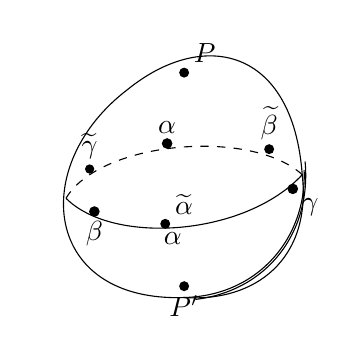
\begin{tikzpicture}[scale=1.2]
\draw (0,0) .. controls (-1.5,-.05) and (-1.65,1.4) .. (-.6,2.2) .. controls (.2,2.85) and (1.15,2.65) .. (1.25,1.3) .. controls (1.35,.4) and (.75,-.05) .. (0,0);
\draw (-1.25,1.05) .. controls (-.75,.55) and (.65,.65) .. (1.25,1.3);
\draw[dashed] (-1.25,1.05) .. controls (-.9,1.65) and (.7,1.8) .. (1.25,1.3);
\draw (.0,.0) .. controls (.8,.02) and (1.3,.65) .. (1.27,1.35);
\draw (.12,-.02) .. controls (.88,.07) and (1.35,.69) .. (1.28,1.44);
\fill (0,2.38) circle(1.5pt) node[above right]{$P$};
\fill (0,.12) circle(1.5pt) node[below]{$\unsure{P'}$};
\fill (-.18,1.63) circle(1.6pt) node[above]{$\alpha$};
\fill (-1,1.36) circle(1.4pt) node[above]{$\widetilde\gamma$};
\fill (.9,1.57) circle(1.5pt) node[above]{$\widetilde\beta$};
\fill (-.95,.91) circle(1.6pt) node[below]{$\beta$};
\fill (-.2,.78) circle(1.5pt) node[above right]{$\widetilde\alpha$};
\node[below] at(-.12,.79){$\deleted{\unsure{\alpha}}$};
\fill (1.15,1.15) circle(1.6pt) node[below right]{$\gamma$};
\end{tikzpicture}}
\margin{De façon générale, on \unsure{désignera|désigne} par $\unsure{P'|x'}$ l'\unsure{antipodique} d'un pt $P$ de $\Sigma$.}
On pose
\[
(3)\qquad\Sigma^*\deleted{\unsure{(I)}}=\Sigma_I\deleted{\unsure{\alpha(I)}}=\Sigma-\deleted{\unsure{\{}}J
\]
On a des iso. canoniques (sur $\mathbb C$)
\[
(4)\quad\left\{\begin{aligned}
M_{0,I}&\simeq\Sigma_I^*\\
\widehat M_{0,I}&\simeq\Sigma_I
\end{aligned}\right.
\]
\mspage{15}
